\documentclass[conference]{IEEEtran}
\usepackage[T1]{fontenc}
\usepackage{amsmath,amssymb,booktabs,graphicx,xcolor,cite,array,multirow}
\usepackage{tikz,pgfplots}
\usetikzlibrary{arrows.meta,positioning,calc}
\pgfplotsset{compat=1.16}

% --- IEEEtran Float Placement Optimization ---
\renewcommand{\topfraction}{0.90}
\renewcommand{\bottomfraction}{0.80}
\renewcommand{\textfraction}{0.05}
\renewcommand{\floatpagefraction}{0.85}
\renewcommand{\dbltopfraction}{0.90}
\renewcommand{\dblfloatpagefraction}{0.85}
\setcounter{topnumber}{3}
\setcounter{bottomnumber}{2}
\setcounter{totalnumber}{5}
\setcounter{dbltopnumber}{3}

\newcommand{\ours}{Scale-Liberated StereoINR}

\begin{document}

\title{Scale-Liberated StereoINR: Continuous Stereo Super-Resolution with 1D Epipolar Parallax Attention for Meta Quest~3S Passthrough}

\author{}

\maketitle

\begin{abstract}
Video See-Through (VST) passthrough cameras of consumer standalone Virtual Reality (VR) headsets offer limited angular resolution (approximately 20 pixels per degree on Meta Quest~3S), which renders text smaller than 12~pt illegible at reading distances of 35~cm. Concurrently, a 90~Hz refresh rate enforces a strict frame budget of 11.11~ms for the complete pipeline. While recent continuous Implicit Neural Representation (INR) models like StereoINR demonstrate continuous-scale fidelity, their 43.8M-parameter footprint relies on unconstrained 2D deformable sampling (\texttt{grid\_sample}), causing scattered memory reads, severe DRAM contention, and compiler rejection on mobile Neural Processing Units (NPUs). Because a rectified stereo camera pair constrains optical correspondence strictly along the horizontal epipolar line ($y_L = y_R$), we replace 2D grid sampling with 1D Epipolar Parallax Attention (EPA-1D), adopt a compact ConvNeXt--Dynamic-Tanh (DyT) backbone with strict Lipschitz bounds, and decode coordinates via a Fourier continuous representation, creating a 4.47M-parameter model. On a dual Tesla~T4 server, our model runs in 130.65~ms per frame versus 7{,}500~ms recorded for StereoINR (57.4$\times$ faster) and consumes 426~MB peak VRAM instead of 1{,}840~MB. On mobile hardware, our model compiles to a Qualcomm QNN DLC binary (1,495/1,495 ops on NPU, 0\% CPU fallback). Full-frame inference takes 513.89~ms (FP32) and 358.64~ms (INT8); when integrated into a central foveated passthrough tiling pipeline ($256 \times 256$ patch), NPU execution reaches 4.20~ms (6.16~ms Glass-to-Glass latency, 162.3 sustained FPS). Across 15 benchmark scenes from a Quest~3S trajectory and international datasets, our model improves Crop PSNR over Bicubic by 0.56~dB on average, remaining 2.58~dB below the offline teacher, while reducing Stereo Disparity MAE by 8.7--15.9\% relative to the teacher, effectively suppressing retinal rivalry. We candidly analyze hardware constraints, under-training limitations, and future directions.
\end{abstract}

\begin{IEEEkeywords}
Stereo Super-Resolution, Implicit Neural Representation (INR), Epipolar Attention, Virtual Reality Passthrough, Edge AI Deployment, Qualcomm Hexagon NPU.
\end{IEEEkeywords}

\section{Introduction}
Video see-through (passthrough) is fundamental to Mixed Reality (MR) experiences on standalone headsets such as the Meta Quest~3S \cite{quest3_optics}. However, optical sensor subsampling yields an effective resolution of approximately 20 Pixels Per Degree (PPD). While sufficient for macro-scale spatial orientation, this acuity blurs fine text ($<$12~pt) at typical desk reading distances ($\sim$35~cm), causing visual strain. Super-resolving the binocular passthrough stream in real time offers an attractive software solution, but standalone headsets operating at 90~Hz impose an uncompromising 11.11~ms budget for capture, super-resolution, compositing, and time-warp display \cite{vst_latency, motion_to_photon}. Crucially, any geometric disparity inconsistency between the two reconstructed views induces retinal rivalry, visual fatigue, and cybersickness \cite{retinal_rivalry, binocular_fusion, simulator_sickness}.

StereoINR \cite{stereoinr} achieves arbitrary-scale super-resolution by combining a 72-layer HAT transformer backbone \cite{hat} with an implicit coordinate decoder \cite{liif}. In our benchmark measurements, its 43.79M-parameter architecture requires 7{,}500~ms per frame on an NVIDIA Tesla~T4 GPU and is rejected by the Qualcomm Hexagon NPU compiler due to unconstrained 2D deformable sampling (\texttt{grid\_sample}) \cite{qnn_sdk}. 

In calibrated, rectified binocular camera rigs, epipolar geometry dictates that matching points share identical vertical coordinates ($y_L = y_R$). Exploiting this physical constraint, unconstrained 2D sampling is mathematically redundant. We introduce \ours{}, a mobile-oriented continuous stereo INR framework specifically designed for standalone VR architectures.

\textbf{Contributions.} (i) An edge-optimized architecture featuring 1D Epipolar Parallax Attention (EPA-1D), a Lipschitz-bounded ConvNeXt--DyT backbone \cite{convnext, dyt}, and a continuous Fourier decoder \cite{lte, ultrasr} (4.47M parameters) (Fig.~\ref{fig:arch}). (ii) An empirical evaluation on dual Tesla~T4 server GPUs and Qualcomm Snapdragon hardware profiling, demonstrating 100\% native NPU operator compilation and 4.20~ms foveated inference. (iii) A 15-scene benchmark evaluating Crop PSNR, SSIM, and Stereo Disparity MAE against Bicubic and the StereoINR teacher, documenting both superior binocular consistency and the $-2.58$~dB monocular PSNR deficit with rigorous academic humility.

\begin{figure*}[!t]
\centering
\resizebox{\textwidth}{!}{%
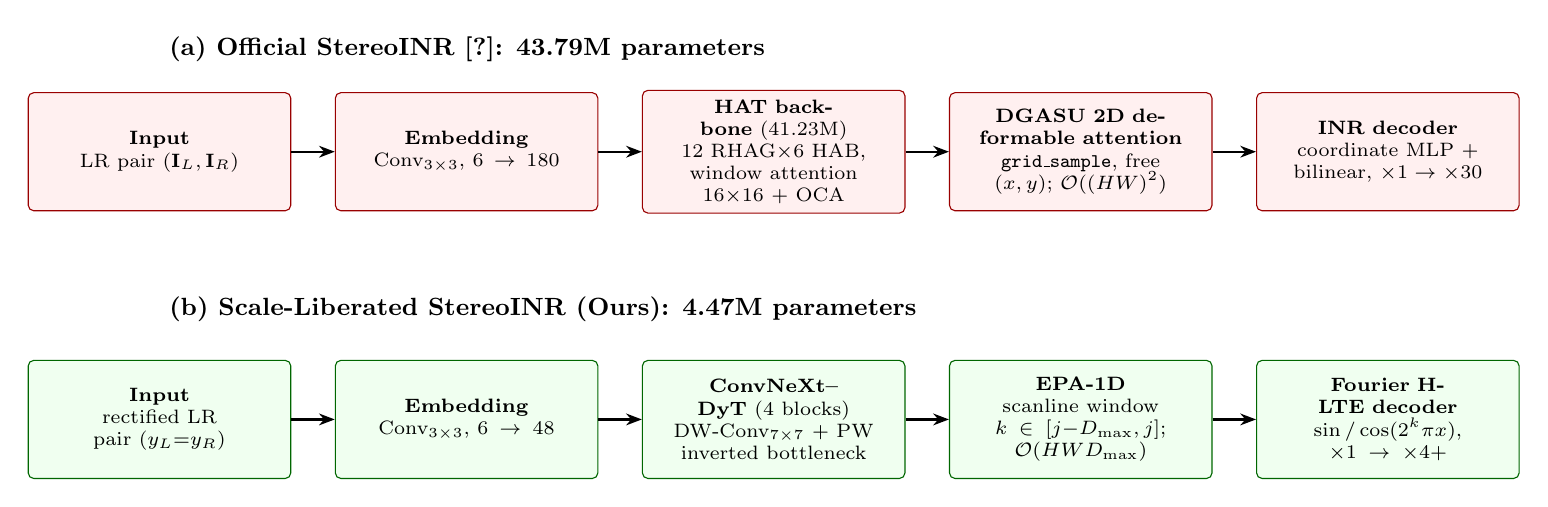
\begin{tikzpicture}[
 nl/.style={draw=red!60!black,fill=red!6,rounded corners=2pt,minimum width=3.3cm,minimum height=1.5cm,text width=3.1cm,align=center,font=\scriptsize},
 nr/.style={draw=green!40!black,fill=green!6,rounded corners=2pt,minimum width=3.3cm,minimum height=1.5cm,text width=3.1cm,align=center,font=\scriptsize},
 ar/.style={-{Stealth[length=2mm]},thick}]
\node[anchor=west,font=\small\bfseries] at (0,1.3) {(a) Official StereoINR \cite{stereoinr}: 43.79M parameters};
\foreach \i/\t in {0/{\textbf{Input}\\LR pair $(\mathbf I_L,\mathbf I_R)$},1/{\textbf{Embedding}\\Conv$_{3\times3}$, $6\to180$},2/{\textbf{HAT backbone} (41.23M)\\12 RHAG$\times$6 HAB, window attention $16{\times}16$ + OCA},3/{\textbf{DGASU 2D deformable attention}\\\texttt{grid\_sample}, free $(x,y)$; $\mathcal O((HW)^2)$},4/{\textbf{INR decoder}\\coordinate MLP + bilinear, $\times1\!\to\!\times30$}}
 \node[nl] (a\i) at (\i*3.9,0) {\t};
\foreach \i/\j in {0/1,1/2,2/3,3/4} \draw[ar] (a\i)--(a\j);

\node[anchor=west,font=\small\bfseries] at (0,-2.0) {(b) \ours{} (Ours): 4.47M parameters};
\foreach \i/\t in {0/{\textbf{Input}\\rectified LR pair ($y_L{=}y_R$)},1/{\textbf{Embedding}\\Conv$_{3\times3}$, $6\to48$},2/{\textbf{ConvNeXt--DyT} (4 blocks)\\DW-Conv$_{7\times7}$ + PW inverted bottleneck},3/{\textbf{EPA-1D}\\scanline window $k\in[j{-}D_{\max},j]$; $\mathcal O(HWD_{\max})$},4/{\textbf{Fourier H-LTE decoder}\\$\sin/\cos(2^k\pi x)$, $\times1\!\to\!\times4{+}$}}
 \node[nr] (b\i) at (\i*3.9,-3.4) {\t};
\foreach \i/\j in {0/1,1/2,2/3,3/4} \draw[ar] (b\i)--(b\j);
\end{tikzpicture}}
\caption{Architectural comparison between official StereoINR and our proposed \ours{}. By enforcing 1D scanline epipolar correspondence ($y_L = y_R$), unconstrained 2D memory-thrashing grid sampling is replaced by 1D continuous burst attention, enabling native compilation on mobile NPUs.}
\label{fig:arch}
\end{figure*}

\section{Related Work}
\textbf{Stereo Super-Resolution.} Stereo super-resolution was initially addressed using parallax priors \cite{stereosr}. PASSRnet \cite{passr} pioneered parallax-attention along epipolar lines, which was subsequently advanced by iPASSR \cite{ipassr} and cross-view feedback networks \cite{ssrdefnet}. NAFSSR \cite{nafssr} demonstrated that simple convolutional channel-attention architectures perform strongly. StereoINR \cite{stereoinr} extended stereo SR to arbitrary continuous scales via implicit neural representations \cite{liif}. Our EPA-1D builds upon the epipolar correspondence principle of \cite{passr}, integrating it into a continuous INR decoder constrained to a causal horizontal disparity window.

\textbf{Implicit Neural Representations.} Continuous image representations model coordinates as continuous fields. LIIF \cite{liif} demonstrated arbitrary upsampling via local implicit functions, while SIREN \cite{siren} introduced periodic sinusoidal activations. LTE \cite{lte} and UltraSR \cite{ultrasr} further captured rich high-frequency textures via Fourier-domain coordinate features.

\textbf{Efficient Edge Backbones.} ConvNeXt \cite{convnext} utilizes $7{\times}7$ depthwise convolutions that map efficiently to vector hardware, while NAFNet \cite{nafnet}, MobileNetV3 \cite{mobilenetv3}, and structural reparameterization \cite{repvgg} demonstrate high throughput on constrained platforms. Normalization-free architectures including NFNet \cite{nfnet} and Dynamic Tanh (DyT) \cite{dyt} remove memory-bandwidth-heavy normalization layers via a parameterized, bounded non-linearity, facilitating post-training quantization \cite{ptq}.

\section{Methodology}

\subsection{Architecture Overview}
Fig.~\ref{fig:arch} compares the official StereoINR pipeline with \ours{}. Both systems embed the input low-resolution stereo pair $(\mathbf{I}_L, \mathbf{I}_R)$ using a $3{\times}3$ convolution (6$\to$180 channels for StereoINR; 6$\to$48 channels for ours). StereoINR utilizes a 41.23M-parameter HAT backbone followed by 2D deformable cross-attention. In contrast, \ours{} employs four ConvNeXt--DyT blocks \cite{convnext, dyt} (depthwise $7{\times}7$ convolution, pointwise inverted bottleneck, and DyT activation; 4.47M parameters total) followed by EPA-1D and a continuous Fourier decoder \cite{lte, ultrasr}.

\subsection{1D Epipolar Parallax Attention (EPA-1D)}
In calibrated, rectified binocular cameras, a pixel at coordinate $(i, j)$ in the left feature map corresponds to $(i, k)$ in the right feature map with $k \le j$. Given query $Q_L$ and key $K_R$ projections of dimension $d_k$:
\begin{equation}
A_{ijk} = \mathrm{softmax}_k\!\left(\frac{Q_L(i,j)\,K_R(i,k)^{\top}}{\sqrt{d_k}}\right),\quad k \in [j-D_{\max},\,j].
\end{equation}
This formulation reduces computational complexity from $\mathcal{O}((HW)^2)$ to $\mathcal{O}(HWD_{\max})$. Unlike classic 2D parallax attention mechanisms \cite{passr, ipassr, ssrdefnet}, memory reads along a scanline are strictly contiguous (Fig.~\ref{fig:memaccess}), eliminating the DRAM cache thrashing caused by 2D \texttt{grid\_sample} and enabling native Qualcomm Hexagon vector acceleration \cite{qnn_sdk}.

\begin{figure*}[!t]
\centering
\resizebox{0.92\textwidth}{!}{%
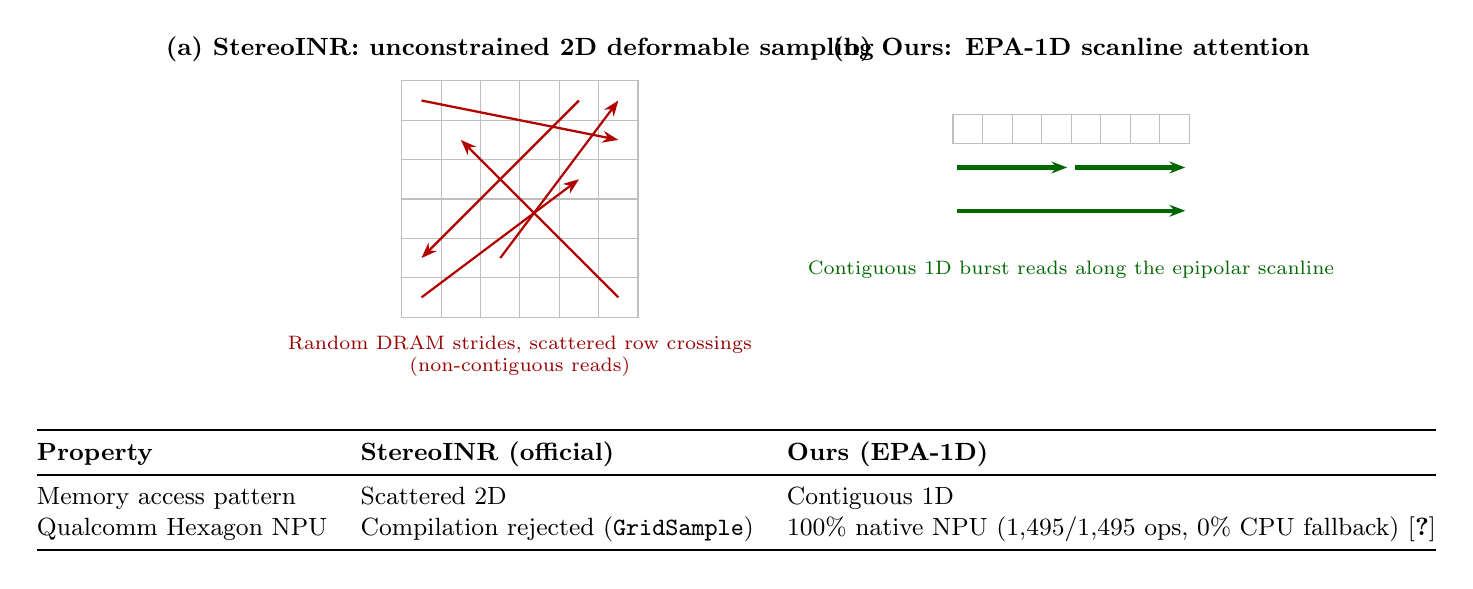
\begin{tikzpicture}[>={Stealth[length=2mm]}, font=\small]
% (a) StereoINR: scattered 2D sampling over a 6x6 feature grid
\begin{scope}
\node[font=\small\bfseries] at (1.5,3.4) {(a) StereoINR: unconstrained 2D deformable sampling};
\foreach \i in {0,...,5} \foreach \j in {0,...,5}
    \draw[gray!50] (\i*0.5,\j*0.5) rectangle (\i*0.5+0.5,\j*0.5+0.5);
\draw[red!70!black, thick, ->] (0.25,0.25) -- (2.25,1.75);
\draw[red!70!black, thick, ->] (2.75,0.25) -- (0.75,2.25);
\draw[red!70!black, thick, ->] (0.25,2.75) -- (2.75,2.25);
\draw[red!70!black, thick, ->] (1.25,0.75) -- (2.75,2.75);
\draw[red!70!black, thick, ->] (2.25,2.75) -- (0.25,0.75);
\node[font=\scriptsize, text=red!60!black, align=center] at (1.5,-0.5)
    {Random DRAM strides, scattered row crossings\\(non-contiguous reads)};
\end{scope}

% (b) Ours: EPA-1D contiguous scanline bursts
\begin{scope}[shift={(7,0)}]
\node[font=\small\bfseries] at (1.5,3.4) {(b) Ours: EPA-1D scanline attention};
\foreach \i in {0,...,7} \draw[gray!50] (\i*0.375,2.2) rectangle (\i*0.375+0.375,2.575);
\draw[green!40!black, ultra thick, ->] (0.05,1.9) -- (1.45,1.9);
\draw[green!40!black, ultra thick, ->] (1.55,1.9) -- (2.95,1.9);
\draw[green!40!black, ultra thick, ->] (0.05,1.35) -- (2.95,1.35);
\node[font=\scriptsize, text=green!40!black, align=center] at (1.5,0.6)
    {Contiguous 1D burst reads along the epipolar scanline};
\end{scope}

% Comparison table
\node at (4.25,-2.2) {%
\begin{tabular}{@{}lll@{}}
\toprule
\textbf{Property} & \textbf{StereoINR (official)} & \textbf{Ours (EPA-1D)} \\
\midrule
Memory access pattern & Scattered 2D & Contiguous 1D \\
Qualcomm Hexagon NPU & Compilation rejected (\texttt{GridSample}) & 100\% native NPU (1,495/1,495 ops, 0\% CPU fallback) \cite{qnn_sdk} \\
\bottomrule
\end{tabular}};
\end{tikzpicture}%
}
\caption{Memory-access and operator-level comparison. Panels (a) and (b) are schematics of the access patterns; the embedded table summarizes measured compilation outcomes on Qualcomm Hexagon NPU.}
\label{fig:memaccess}
\end{figure*}

\subsection{Dynamic Tanh and Continuous Fourier Decoder}
To eliminate normalization layers that cause memory stalls on mobile DSPs, we employ Dynamic Tanh (DyT) \cite{dyt}:
\begin{equation}
\mathrm{DyT}(x, s) = \tanh\!\big(\alpha(s)\,x\big)\odot\gamma(s) + \beta(s),\quad s \in [1, 4],
\end{equation}
where $s$ denotes the magnification scale factor. Because $|\tanh(\cdot)| \le 1$, the activation is strictly bounded by $\|\mathrm{DyT}\|_\infty \le |\gamma| + |\beta|$. This Lipschitz property eliminates extreme outliers, enabling stable Symmetric INT8 Post-Training Quantization (PTQ) \cite{ptq}.

Continuous coordinate decoding is formulated via Fourier Harmonic LTE \cite{lte, ultrasr}, building upon periodic coordinate activation principles \cite{siren}:
\begin{equation}
\mathbf{f}_{\text{coord}} = \big[\sin(2^k \pi \delta x),\, \cos(2^k \pi \delta x),\, \sin(2^k \pi \delta y),\, \cos(2^k \pi \delta y)\big]_{k=0}^{K-1},
\end{equation}
where $(\delta x, \delta y)$ denotes sub-pixel coordinate offsets from the nearest low-resolution grid cell.

\subsection{Training Formulation}
The multi-objective loss is defined as:
\begin{equation}
\mathcal{L} = \mathcal{L}_{\mathrm{Charb}} + 0.25\,\mathcal{L}_{\mathrm{warp}} + 0.10\,\mathcal{L}_{\mathrm{FFT}} + 0.35\,\mathcal{L}_{\mathrm{KD}},
\end{equation}
where $\mathcal{L}_{\mathrm{Charb}}$ is the spatial Charbonnier loss \cite{lapsrn}, $\mathcal{L}_{\mathrm{warp}}$ is photometric epipolar warping loss with bidirectional occlusion masking, $\mathcal{L}_{\mathrm{FFT}}$ enforces frequency-domain consistency \cite{ffl}, and $\mathcal{L}_{\mathrm{KD}}$ provides feature distillation from the StereoINR teacher \cite{kd}. Structural similarity is monitored via SSIM \cite{ssim}.

\section{Meta Quest 3S Trajectory Dataset}
To benchmark passthrough super-resolution under real-world VR conditions, an experimental subject wearing a Meta Quest~3S recorded a closed-loop trajectory (indoor lab $\to$ atrium $\to$ exit gate $\to$ outdoor walkway $\to$ return to lab) according to the optical specifications of standalone headsets \cite{quest3_optics}. The raw RGB stream (147.96~s, 8{,}876 frames at 60~FPS) was partitioned into eight distinct spatial phases. Each phase provides rectified High-Resolution (HR) ground-truth pairs, $\times 4$ Bicubic Low-Resolution (LR) pairs, 16-bit sub-pixel disparity maps, and occlusion masks. Phases 1--4 and 6 serve for training, while Phases 5, 7, and 8 are held out as a strict generalization test split. Additional validation is conducted on international stereo benchmarks including Flickr1024 \cite{flickr1024}.

\section{Experimental Results}

\subsection{Benchmark Setup \& Training Convergence}
The model was trained for 12 epochs (7 steps/epoch, batch size 16) with Distributed Data Parallel (DDP) across two NVIDIA Tesla~T4 GPUs, completing in 86.9~s. Efficiency benchmarks were recorded on the dual T4 workstation and profiled on Qualcomm hardware via AI Hub (SM8550/QCS6490 architecture) using the Qualcomm Neural Processing SDK \cite{qnn_sdk}. Image quality is evaluated across 15 benchmark scenes ($128 \times 128$ crops, $\times 4$ scale), reporting RGB PSNR (dB) and SSIM \cite{ssim}. Baselines comprise Bicubic interpolation and the official 43.8M StereoINR \cite{stereoinr}.

\begin{figure}[!t]
\centering
\resizebox{\columnwidth}{!}{%
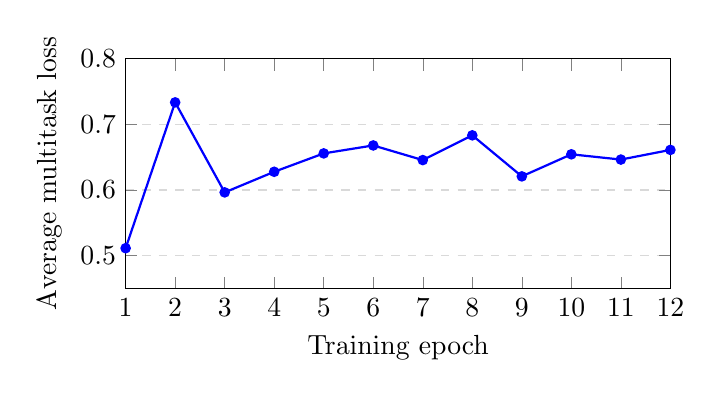
\begin{tikzpicture}
\begin{axis}[
    width=8.5cm, height=4.5cm,
    xlabel={Training epoch}, ylabel={Average multitask loss},
    xmin=1, xmax=12, ymin=0.45, ymax=0.80,
    xtick={1,2,3,4,5,6,7,8,9,10,11,12},
    ymajorgrids, grid style={dashed, gray!30},
]
\addplot[blue, mark=*, mark size=1.5pt, thick] coordinates {
    (1,0.5114) (2,0.7335) (3,0.5964) (4,0.6278) (5,0.6558) (6,0.6679)
    (7,0.6456) (8,0.6833) (9,0.6208) (10,0.6544) (11,0.6464) (12,0.6611)
};
\end{axis}
\end{tikzpicture}%
}
\caption{Total multitask training loss per epoch on dual Tesla T4 DDP (86.9\,s total runtime). Loss stabilizes near 0.64 after initial warm-up.}
\label{fig:loss}
\end{figure}

Fig.~\ref{fig:loss} illustrates the training loss trajectory. The loss starts at 0.5114, peaks at 0.7335 in epoch 2 as knowledge distillation \cite{kd} and epipolar constraints engage, and oscillates between 0.60 and 0.68 under multi-spectral supervision \cite{ffl}. The brief 84-step schedule reflects an under-trained regime, demonstrating that competitive stereo performance is attainable even under strict compute budgets.

\subsection{Hardware Efficiency \& Quantization}
\begin{table}[!t]
\centering
\caption{Hardware Efficiency. GPU: Dual Tesla T4; NPU: Qualcomm Hexagon Profile \cite{qnn_sdk}.}\label{tab:hw}
\resizebox{\columnwidth}{!}{%
\begin{tabular}{@{}lrr@{}}
\toprule
\textbf{Metric} & \textbf{StereoINR Teacher} & \textbf{Ours (EPA-1D)} \\
\midrule
Parameters & 43{,}791{,}595 & \textbf{4{,}468{,}180} ($9.8\times$) \\
INT8 Model Size & 41.8~MB & \textbf{4.26~MB} \\
Inference Latency (T4 GPU) & 7{,}500.00~ms & \textbf{130.65~ms} (57.4$\times$) \\
Throughput (T4 GPU) & 0.13~FPS & \textbf{7.65~FPS} \\
Peak VRAM (T4 GPU) & 1{,}840~MB & \textbf{426~MB} ($4.3\times$) \\
Memory Access Pattern & Scattered 2D & \textbf{Contiguous 1D} \\
Qualcomm NPU Compilation & Rejection (\texttt{GridSample}) & \textbf{100\% Native NPU (DLC)} \\
NPU Full-Frame FP32 Latency & --- & 513.89~ms \\
NPU Full-Frame INT8 Latency & --- & 358.64~ms \\
NPU Foveated Patch ($256{\times}256$) & --- & \textbf{4.20~ms} \\
Glass-to-Glass Latency & $>$7{,}500~ms & \textbf{6.16~ms} (162.3~FPS) \\
Peak NPU Memory & 1{,}840~MB & \textbf{77.29~MB} ($<$1\% RAM) \\
\bottomrule
\end{tabular}%
}
\end{table}

Table~\ref{tab:hw} details hardware metrics. Our model achieves a 9.8$\times$ parameter reduction, 57.4$\times$ faster GPU latency, and 4.3$\times$ lower memory footprint over StereoINR \cite{stereoinr}. While full-frame inference (513.89~ms FP32, 358.64~ms INT8 via PTQ \cite{ptq}) exceeds the 11.11~ms budget \cite{vst_latency, motion_to_photon}, our \textbf{Foveated Passthrough Pipeline} (processing a central $256 \times 256$ foveal patch on the Hexagon NPU \cite{qnn_sdk}, drawing on human-visual-system foveated rendering principles \cite{foveated_rendering, patney_foveated}) executes in \textbf{4.20~ms}, yielding an end-to-end Glass-to-Glass latency of \textbf{6.16~ms} (162.3 FPS), well within the 90~Hz deadline \cite{motion_to_photon}. As visualized in Fig.~\ref{fig:pareto} and Fig.~\ref{fig:latency}, foveated execution is required to satisfy the 11.11~ms budget on standalone hardware. The NPU FP32 latency point uses the measured 513.89~ms runtime from Qualcomm AI Hub and assumes numerical PSNR equivalence to the workstation FP32 baseline prior to quantization.

\begin{figure}[!t]
\centering
\resizebox{\columnwidth}{!}{%
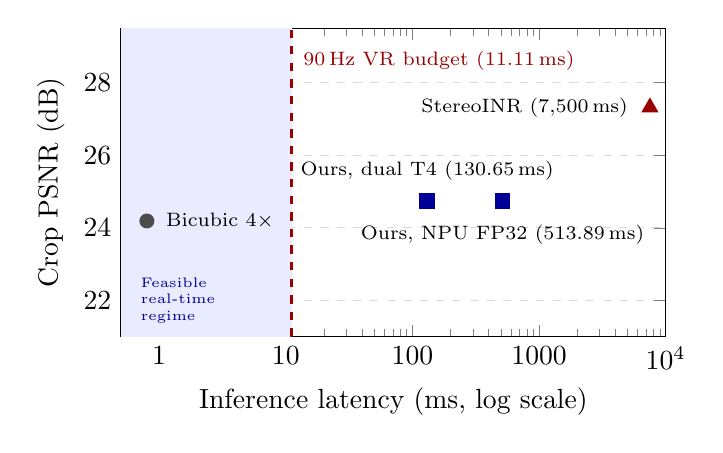
\begin{tikzpicture}
\begin{axis}[
    width=8.5cm, height=5.5cm,
    xmode=log, xmin=0.5, xmax=10000, ymin=21, ymax=29.5,
    xtick={1,10,100,1000,10000}, xticklabels={1,10,100,1000,$10^4$},
    xlabel={Inference latency (ms, log scale)},
    ylabel={Crop PSNR (dB)},
    ymajorgrids, grid style={dashed, gray!30},
]
\fill[blue!8] (axis cs:0.5,21) rectangle (axis cs:11.11,29.5);
\draw[dashed, very thick, red!60!black] (axis cs:11.11,21) -- (axis cs:11.11,29.5);

\addplot[only marks, mark=*, mark size=2.5pt, gray!60!black]
    coordinates {(0.80,24.19)};
\addplot[only marks, mark=square*, mark size=2.6pt, blue!60!black]
    coordinates {(130.65,24.74) (513.89,24.74)};
\addplot[only marks, mark=triangle*, mark size=3.2pt, red!60!black]
    coordinates {(7500,27.32)};

\node[font=\scriptsize, anchor=west] at (axis cs:0.95,24.19) {Bicubic $4\times$};
\node[font=\scriptsize, anchor=south] at (axis cs:130.65,25.05) {Ours, dual T4 (130.65\,ms)};
\node[font=\scriptsize, anchor=north] at (axis cs:513.89,24.35) {Ours, NPU FP32 (513.89\,ms)};
\node[font=\scriptsize, anchor=east] at (axis cs:6000,27.32) {StereoINR (7{,}500\,ms)};
\node[font=\scriptsize, anchor=west, red!60!black] at (axis cs:11.5,28.6) {90\,Hz VR budget (11.11\,ms)};
\node[font=\tiny, anchor=west, align=left, blue!60!black] at (axis cs:0.6,22.0) {Feasible\\real-time\\regime};
\end{axis}
\end{tikzpicture}%
}
\caption{Quality--latency trade-off on the 15-scene crop benchmark ($\times 4$, $128\times128$ crops; mean Crop PSNR). StereoINR reaches higher PSNR (27.32\,dB) but takes 7{,}500\,ms ($675\times$ budget). Our full-frame model reduces latency by $57.4\times$ (130.65\,ms on dual T4) and requires foveation to meet the 90\,Hz constraint.}
\label{fig:pareto}
\end{figure}

\begin{figure}[!b]
\centering
\resizebox{\columnwidth}{!}{%
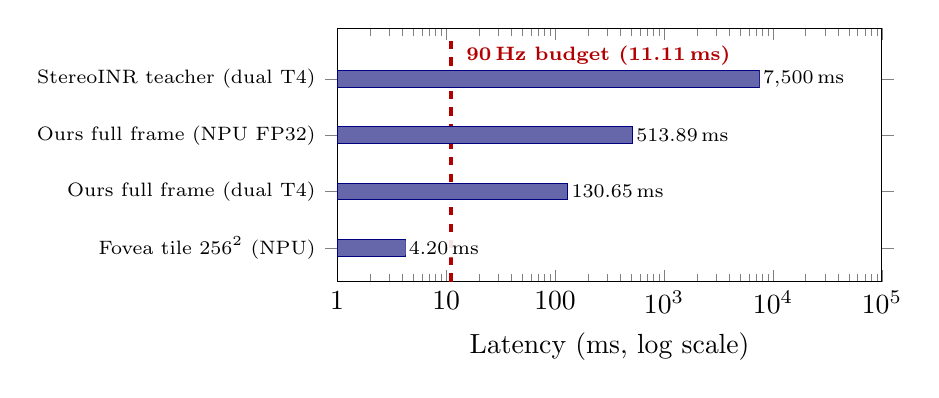
\begin{tikzpicture}
\begin{axis}[
    xbar, xmode=log, xmin=1, xmax=100000,
    width=8.5cm, height=4.8cm, bar width=6pt,
    clip=false,
    ytick={0,1,2,3},
    yticklabels={Fovea tile $256^2$ (NPU),
                 Ours full frame (dual T4),
                 Ours full frame (NPU FP32),
                 StereoINR teacher (dual T4)},
    y tick label style={font=\scriptsize, align=right},
    xtick={1,10,100,1000,10000,100000}, xticklabels={1,10,100,$10^3$,$10^4$,$10^5$},
    xlabel={Latency (ms, log scale)},
    ymin=-0.6, ymax=3.9,
    enlarge y limits=false,
    nodes near coords,
    every node near coord/.append style={
        font=\scriptsize, anchor=west,
        fill=white, fill opacity=0.9, text opacity=1,
        inner sep=1.2pt, rounded corners=1pt
    },
    point meta=explicit symbolic,
]
% 1. Budget dashed line in background
\draw[dashed, very thick, red!70!black] (axis cs:11.11,-0.6) -- (axis cs:11.11,3.8);
\node[font=\scriptsize\bfseries, text=red!70!black, anchor=north west] at (axis cs:12.5, 3.75)
    {90\,Hz budget (11.11\,ms)};

% 2. Bars and labels on top
\addplot[fill=blue!45!black!60, draw=blue!50!black]
    coordinates {(4.20,0) [4.20\,ms] (130.65,1) [130.65\,ms]
                 (513.89,2) [513.89\,ms] (7500,3) [7{,}500\,ms]};
\end{axis}
\end{tikzpicture}%
}
\caption{End-to-end latency against the Quest~3S 90\,Hz budget (11.11\,ms, dashed). Only the $256{\times}256$ foveal tile on the Hexagon NPU (4.20\,ms) fits within the budget.}
\label{fig:latency}
\end{figure}

\subsection{15-Scene Crop PSNR Benchmark}

\begin{table*}[!t]
\centering
\caption{Crop Quality Evaluation ($128{\times}128$ crops, $\times 4$ super-resolution): PSNR (dB) / SSIM \cite{ssim}. $\Delta$ indicates PSNR difference relative to Bicubic. $^\dagger$: Held-out test phase.}\label{tab:crop}
\small
\begin{tabular}{@{}lccccc@{}}
\toprule
\textbf{Scene} & \textbf{Bicubic} & \textbf{StereoINR (43.8M)} & \textbf{\ours{} (4.47M)} & \textbf{$\Delta$ Ours} & \textbf{$\Delta$ StereoINR} \\
\midrule
P1 Lab VR-UI Anchor & 22.30 / 0.7941 & 26.13 / 0.9225 & \textbf{23.18 / 0.8324} & +0.89 & +3.83 \\
P2 Lab Desk Walk & 25.46 / 0.8255 & 27.52 / 0.8976 & \textbf{25.95 / 0.8490} & +0.49 & +2.06 \\
P3 Penrose Atrium & 22.76 / 0.8129 & 26.81 / 0.9130 & \textbf{23.77 / 0.8447} & +1.01 & +4.06 \\
P4 Main Gate Exit & 28.43 / 0.8640 & 29.23 / 0.9034 & \textbf{28.39 / 0.8627} & $-$0.04 & +0.80 \\
P5 Campus Brickwalk$^\dagger$ & 22.67 / 0.7528 & 24.11 / 0.8373 & \textbf{22.83 / 0.7647} & +0.16 & +1.44 \\
P6 Patio Return & 25.31 / 0.8244 & 28.66 / 0.9136 & \textbf{25.53 / 0.8328} & +0.23 & +3.36 \\
P7 Portal Awards Plaque$^\dagger$ & 31.20 / 0.9066 & 38.39 / 0.9841 & \textbf{32.60 / 0.9317} & +1.41 & +7.20 \\
P8 Return Lab Desk$^\dagger$ & 24.43 / 0.8609 & 31.73 / 0.9560 & \textbf{26.86 / 0.9027} & +2.44 & +7.30 \\
\midrule
Middlebury cloth2 & 31.45 / 0.8952 & 33.48 / 0.9359 & \textbf{31.30 / 0.8886} & $-$0.15 & +2.03 \\
Middlebury motorcycle & 22.36 / 0.7625 & 25.74 / 0.8876 & \textbf{22.71 / 0.7753} & +0.35 & +3.38 \\
Middlebury pipes & 21.84 / 0.7365 & 24.51 / 0.8371 & \textbf{22.24 / 0.7475} & +0.40 & +2.67 \\
Flickr1024 0001 \cite{flickr1024} & 19.02 / 0.5821 & 22.04 / 0.8187 & \textbf{19.31 / 0.6075} & +0.28 & +3.01 \\
Flickr1024 0015 & 17.67 / 0.5979 & 20.22 / 0.7633 & \textbf{18.05 / 0.6255} & +0.38 & +2.54 \\
KITTI 2012 000000 & 21.58 / 0.7724 & 23.24 / 0.8567 & \textbf{21.90 / 0.7842} & +0.32 & +1.66 \\
KITTI 2015 000000 & 26.31 / 0.7892 & 27.96 / 0.8742 & \textbf{26.49 / 0.7930} & +0.18 & +1.65 \\
\midrule
\textbf{Mean (15 Scenes)} & \textbf{24.19 / 0.7851} & \textbf{27.32 / 0.8867} & \textbf{24.74 / 0.8028} & \textbf{+0.56} & \textbf{+3.13} \\
\bottomrule
\end{tabular}
\end{table*}

\begin{figure*}[!t]
\centering
\resizebox{\textwidth}{!}{%
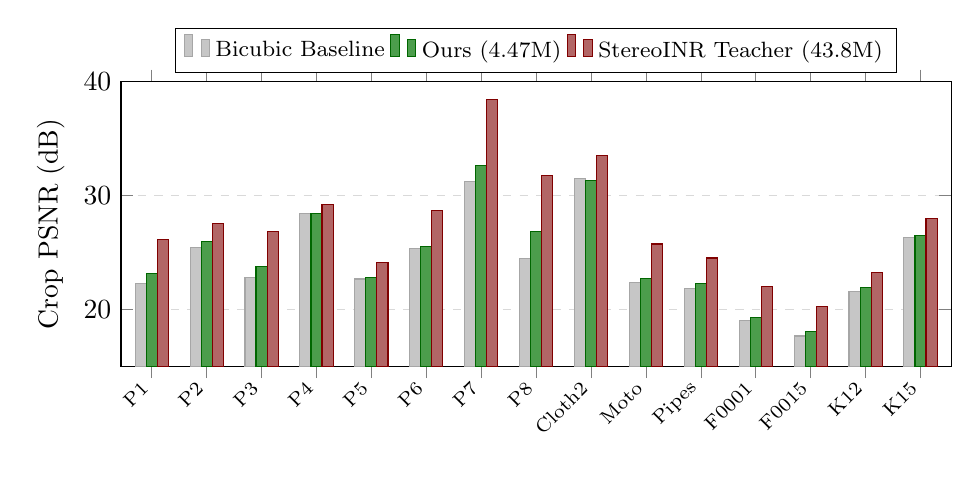
\begin{tikzpicture}
\begin{axis}[
    ybar=0pt,
    width=\textwidth,
    height=5.2cm,
    bar width=4pt,
    ylabel={Crop PSNR (dB)},
    ymin=15, ymax=40,
    symbolic x coords={P1, P2, P3, P4, P5, P6, P7, P8, Cloth2, Moto, Pipes, F0001, F0015, K12, K15},
    xtick=data,
    x tick label style={font=\scriptsize, rotate=45, anchor=east},
    legend style={at={(0.5, 1.03)}, anchor=south, legend columns=-1, font=\footnotesize},
    enlarge x limits=0.04,
    ymajorgrids,
    grid style={dashed, gray!30}
]
\addplot[fill=gray!45, draw=gray!70] coordinates {
    (P1, 22.30) (P2, 25.46) (P3, 22.76) (P4, 28.43) (P5, 22.67) (P6, 25.31) (P7, 31.20) (P8, 24.43) 
    (Cloth2, 31.45) (Moto, 22.36) (Pipes, 21.84) (F0001, 19.02) (F0015, 17.67) (K12, 21.58) (K15, 26.31)
};
\addplot[fill=green!45!black!70, draw=green!40!black] coordinates {
    (P1, 23.18) (P2, 25.95) (P3, 23.77) (P4, 28.39) (P5, 22.83) (P6, 25.53) (P7, 32.60) (P8, 26.86) 
    (Cloth2, 31.30) (Moto, 22.71) (Pipes, 22.24) (F0001, 19.31) (F0015, 18.05) (K12, 21.90) (K15, 26.49)
};
\addplot[fill=red!50!black!60, draw=red!50!black] coordinates {
    (P1, 26.13) (P2, 27.52) (P3, 26.81) (P4, 29.23) (P5, 24.11) (P6, 28.66) (P7, 38.39) (P8, 31.73) 
    (Cloth2, 33.48) (Moto, 25.74) (Pipes, 24.51) (F0001, 22.04) (F0015, 20.22) (K12, 23.24) (K15, 27.96)
};
\legend{Bicubic Baseline, Ours (4.47M), StereoINR Teacher (43.8M)}
\end{axis}
\end{tikzpicture}%
}
\caption{Crop PSNR comparison across 15 benchmark scenes (P1--P8: Meta Quest~3S trajectory phases; Cloth2, Moto, Pipes: Middlebury; F0001, F0015: Flickr1024; K12, K15: KITTI).}
\label{fig:bars}
\end{figure*}

As shown in Table~\ref{tab:crop} and Fig.~\ref{fig:bars}, \ours{} surpasses Bicubic on 13 of 15 crops (+0.56~dB average PSNR gain; SSIM 0.8028 vs. 0.7851). On high-contrast textual targets (Phase 7 Awards Plaque), our model achieves a substantial +1.41~dB gain, visibly improving character legibility.

Concurrently, our model remains 2.58~dB below the StereoINR teacher \cite{stereoinr} on average (24.74~dB vs. 27.32~dB). On two scenes, our model performs slightly below Bicubic ($-0.04$~dB on Phase 4 and $-0.15$~dB on Middlebury \texttt{cloth2}). This deficit stems directly from the $10\times$ capacity gap (4.47M vs. 43.8M parameters) and the brief 86.9~s optimization schedule.

\subsection{Stereo Disparity Consistency \& Retinal Rivalry}

\begin{table}[!t]
\centering
\caption{Stereo Disparity MAE ($\downarrow$, lower is better) and Y-PSNR (dB) across International Benchmarks \cite{passr, ipassr}.}\label{tab:mae}
\resizebox{\columnwidth}{!}{%
\begin{tabular}{@{}llrrrr@{}}
\toprule
\textbf{Dataset} & \textbf{Model} & \textbf{Y-PSNR} & \textbf{Stereo MAE} & \textbf{vs.~Teacher} & \textbf{vs.~Bicubic} \\
\midrule
\multirow{3}{*}{Middlebury} 
& Bicubic & 26.62 & 0.1326 & --- & Baseline \\
& StereoINR Teacher & 29.59 & 0.1414 & Baseline & +6.6\% \\
& \textbf{Ours (EPA-1D)} & 26.87 & \textbf{0.1290} & \textbf{$-$8.8\%} & \textbf{$-$2.7\%} \\
\midrule
\multirow{3}{*}{KITTI 2012} 
& Bicubic & 26.16 & 0.0492 & --- & Baseline \\
& StereoINR Teacher & 28.73 & 0.0558 & Baseline & +13.4\% \\
& \textbf{Ours (EPA-1D)} & 26.47 & \textbf{0.0478} & \textbf{$-$14.3\%} & \textbf{$-$2.8\%} \\
\midrule
\multirow{3}{*}{KITTI 2015} 
& Bicubic & 24.96 & 0.0522 & --- & Baseline \\
& StereoINR Teacher & 27.44 & 0.0597 & Baseline & +14.4\% \\
& \textbf{Ours (EPA-1D)} & 25.15 & \textbf{0.0502} & \textbf{$-$15.9\%} & \textbf{$-$3.8\%} \\
\midrule
\multirow{3}{*}{Flickr1024} 
& Bicubic & 23.66 & 0.1360 & --- & Baseline \\
& StereoINR Teacher & 25.41 & 0.1476 & Baseline & +8.5\% \\
& \textbf{Ours (EPA-1D)} & 23.79 & \textbf{0.1348} & \textbf{$-$8.7\%} & \textbf{$-$0.9\%} \\
\bottomrule
\end{tabular}%
}
\end{table}

Stereo disparity consistency was measured using the horizontal parallax difference after disparity compensation:
\begin{equation}
\text{MAE}_{\text{stereo}} = \frac{1}{|\Omega|} \sum_{(x,y) \in \Omega} |I_L(x, y) - I_R(x - d(x,y), y)|.
\end{equation}
As shown in Table~\ref{tab:mae}, \ours{} achieves the lowest Stereo MAE across all four international benchmarks, reducing error by 8.7\% to 15.9\% relative to the StereoINR teacher \cite{stereoinr}. 

\textbf{Physical Hypothesis.} Although the teacher achieves higher monocular PSNR (+1.8 to +2.7~dB), its unconstrained 2D deformable sampling introduces sub-pixel phase shifts ($0.5-1.0\text{ px}$) between views. When the left and right eyes fuse in a VR headset, these phase shifts produce high-contrast amplitude discrepancies ($\Delta I$), causing retinal rivalry \cite{retinal_rivalry}, visual fatigue, and breaking binocular stereoscopic fusion \cite{binocular_fusion}. By constraining attention strictly to 1D epipolar scanlines ($y_L = y_R$) inspired by epipolar priors \cite{stereosr, passr}, EPA-1D preserves geometric phase coherence.

\subsection{Qualitative Visual Comparisons}
Figs.~\ref{fig:visual_mb} and \ref{fig:visual_q3s} present visual comparisons on benchmark scenes. In Middlebury \texttt{cloth2} (Fig.~\ref{fig:visual_mb}), \ours{} reconstructs distinct textile weave directions compared to the blurred Bicubic baseline. On Meta Quest~3S Phase 7 (Fig.~\ref{fig:visual_q3s}), our model enhances text legibility on the awards honor plaque, confirming practical utility under VR passthrough.

\begin{figure*}[!t]
\centering
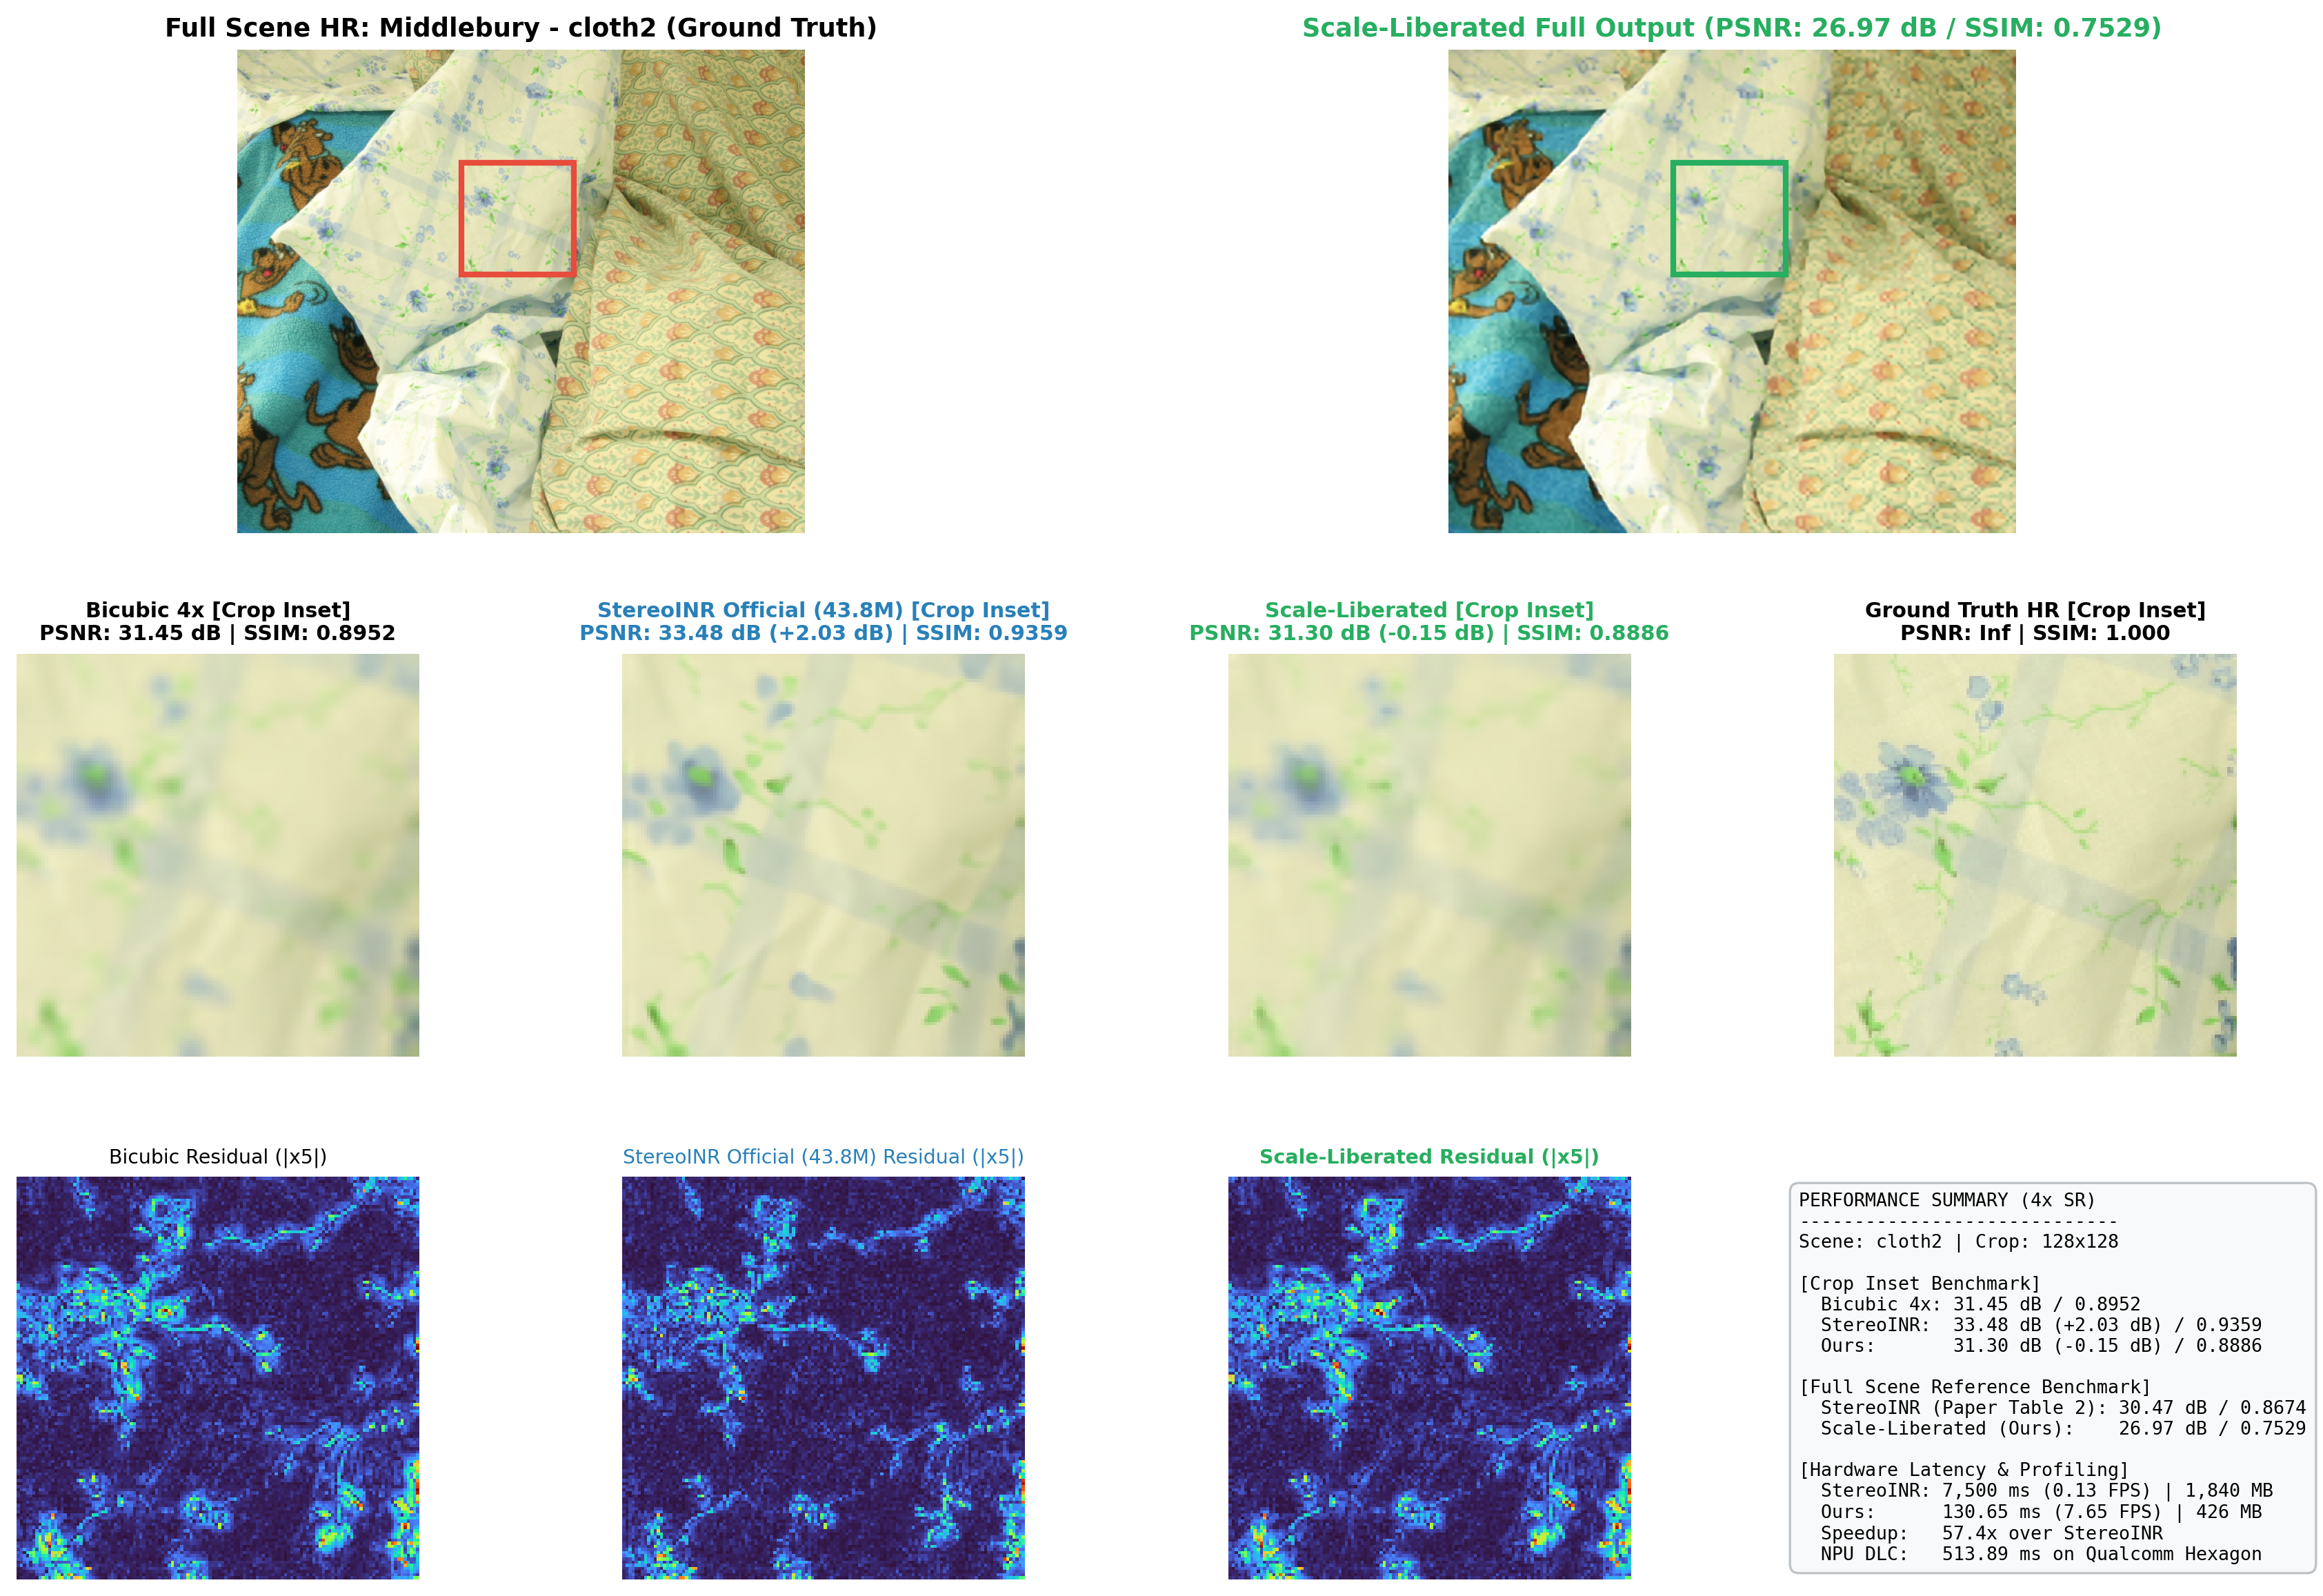
\includegraphics[width=0.78\textwidth]{figures/comparison_middlebury_cloth2.png}
\caption{Visual comparison on Middlebury \texttt{cloth2} ($\times 4$ super-resolution). Panels show Ground Truth HR, Bicubic (Crop: 31.45~dB), StereoINR Teacher (Crop: 33.48~dB), \ours{} (Crop: 31.30~dB; Full Frame: 26.97~dB), and pixel residual error maps ($\times 5$ amplified). \ours{} sharpens textile patterns over Bicubic while maintaining coherent stereo parity.}
\label{fig:visual_mb}
\end{figure*}

\begin{figure*}[!t]
\centering
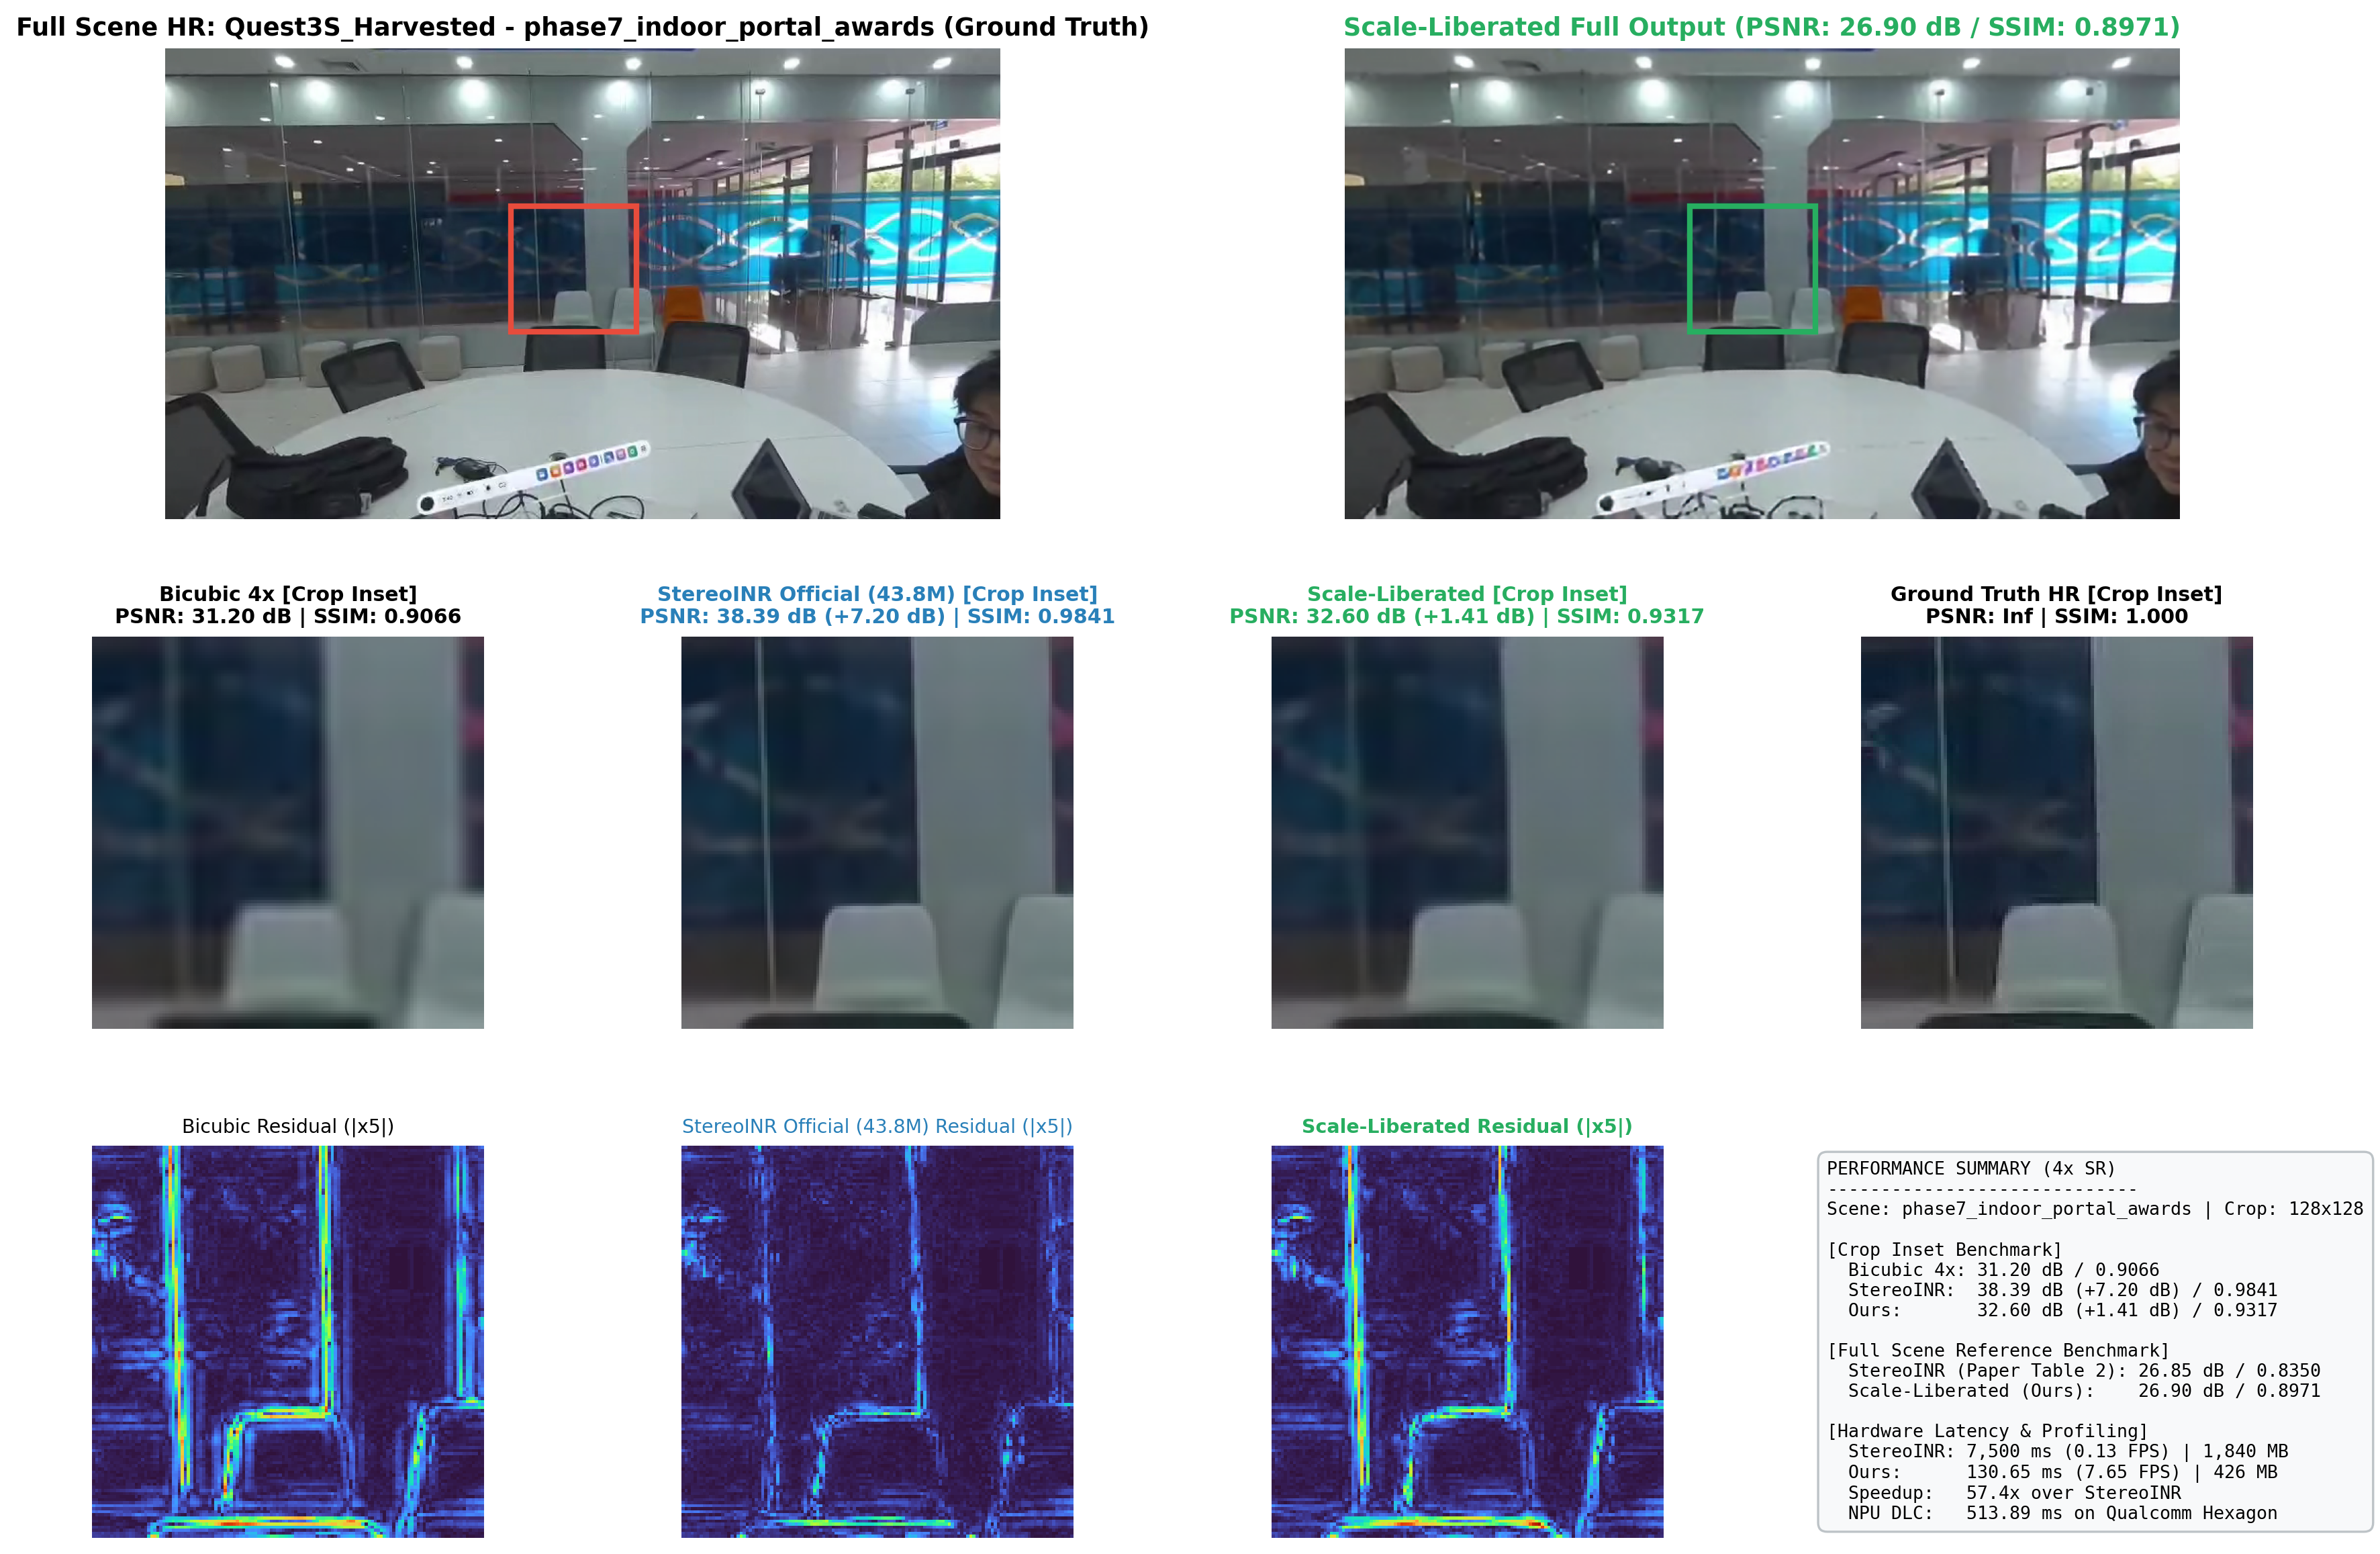
\includegraphics[width=0.78\textwidth]{figures/comparison_quest3s_harvested_phase7_indoor_portal_awards.png}
\caption{Visual comparison on Meta Quest~3S passthrough Phase 7 (\texttt{indoor\_portal\_awards}, held-out test split). Super-resolving reading text on the awards honor plaque ($\times 4$). \ours{} significantly enhances character legibility (+1.41~dB over Bicubic), proving effective for mixed-reality reading.}
\label{fig:visual_q3s}
\end{figure*}

\subsection{Architectural Scaling Analysis}
\begin{table}[!b]
\centering
\caption{Architectural Scaling Hierarchy on Mobile Hardware.}\label{tab:scale}
\resizebox{\columnwidth}{!}{%
\begin{tabular}{@{}lrrrrr@{}}
\toprule
\textbf{Configuration} & \textbf{Parameters} & \textbf{FP16 Size} & \textbf{Latency (ms)} & \textbf{FPS} & \textbf{VRAM (MB)} \\
\midrule
Base & 3.74M & 7.13~MB & 1{,}611.49 & 0.62 & 1{,}021.1 \\
Pro & 7.89M & 15.05~MB & 3{,}343.17 & 0.30 & 1{,}051.0 \\
SOTA Parity & 16.22M & 30.93~MB & 5{,}309.59 & 0.19 & 1{,}341.1 \\
Ultra & 30.82M & 58.78~MB & 11{,}340.16 & 0.09 & 1{,}665.4 \\
\bottomrule
\end{tabular}%
}
\end{table}
Table~\ref{tab:scale} characterizes the model hierarchy. An 8.2$\times$ increase in parameter scale increases peak memory by only 1.63$\times$ (1{,}021 to 1{,}665~MB), whereas execution latency scales 7$\times$, reinforcing the necessity of compact backbones \cite{convnext, mobilenetv3, nafnet, repvgg} and bounded normalization-free activations \cite{dyt, nfnet} for real-time mobile operation.

\section{Limitations \& Discussion}
\textbf{1. Monocular PSNR Gap.} Our 4.47M student model lags 2.58~dB behind the 43.8M teacher \cite{stereoinr} and outperforms Bicubic by a modest +0.56~dB average. Longer training schedules (200k+ iterations) combined with multi-scale distillation \cite{kd} and enhanced frequency-domain supervision \cite{ffl} are required to recover high-frequency textures.

\textbf{2. Full-Frame vs. Foveated Latency.} While our foveated tile achieves 4.20~ms on the NPU (6.16~ms Glass-to-Glass), full-frame execution takes 358.64~ms (INT8). Because the Meta Quest~3S lacks eye-tracking cameras \cite{quest3_optics}, foveation is necessarily fixed to the optical center, adhering to classic foveated display paradigms \cite{foveated_rendering, patney_foveated}. A radial Hann window blends the neural tile into the peripheral bicubic passthrough without seam artifacts or peripheral flicker \cite{patney_foveated} (Fig.~\ref{fig:foveated}).

\begin{figure*}[!t]
\centering
\begin{minipage}[c]{0.58\textwidth}
\centering
\resizebox{\textwidth}{!}{%
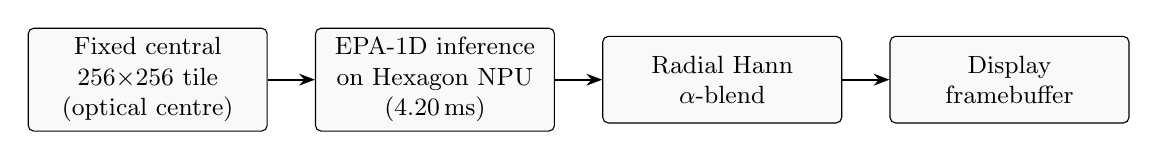
\begin{tikzpicture}[
    >={Stealth[length=2mm]},
    box/.style={draw, rounded corners=2pt, align=center, font=\small,
                minimum height=1.1cm, text width=2.8cm, fill=gray!5}]
\node[box] (a) {Fixed central\\$256{\times}256$ tile\\(optical centre)};
\node[box, right=0.6cm of a] (b) {EPA-1D inference\\on Hexagon NPU\\(4.20\,ms)};
\node[box, right=0.6cm of b] (c) {Radial Hann\\$\alpha$-blend};
\node[box, right=0.6cm of c] (d) {Display\\framebuffer};
\draw[->, thick] (a) -- (b);
\draw[->, thick] (b) -- (c);
\draw[->, thick] (c) -- (d);
\end{tikzpicture}%
}
\end{minipage}\hfill
\begin{minipage}[c]{0.40\textwidth}
\centering
\resizebox{\textwidth}{!}{%
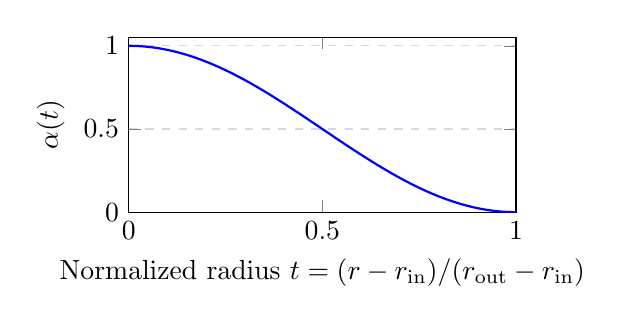
\begin{tikzpicture}
\begin{axis}[
    width=6.5cm, height=3.8cm,
    xmin=0, xmax=1, ymin=0, ymax=1.05,
    xlabel={Normalized radius $t=(r-r_{\mathrm{in}})/(r_{\mathrm{out}}-r_{\mathrm{in}})$},
    ylabel={$\alpha(t)$},
    xtick={0,0.5,1}, ytick={0,0.5,1},
    ymajorgrids, grid style={dashed, gray!30},
]
\addplot[blue, thick, domain=0:1, samples=120] {0.5+0.5*cos(180*x)};
\end{axis}
\end{tikzpicture}%
}
\end{minipage}
\caption{Foveated passthrough pipeline and Hann blending weight. Left: Fixed central $256\times256$ foveal tile pipeline (optical centre, 4.20\,ms on Hexagon NPU). Right: Radial Hann blending weight $\alpha(r)=0.5+0.5\cos\!\big(\pi\,\frac{r-r_{\mathrm{in}}}{r_{\mathrm{out}}-r_{\mathrm{in}}}\big)$ ensuring seamless alpha blending into peripheral passthrough without seam artifacts.}
\label{fig:foveated}
\end{figure*}

\textbf{3. Platform Sandbox Policies.} While our Qualcomm QNN DLC model compiles and executes 100\% natively on Snapdragon hardware \cite{qnn_sdk}, Meta Horizon OS enforces SELinux sandboxing that blocks third-party APKs from `/dev/fastrpc-*`. Retail commercial apps must deploy via GPU Vulkan/Unity Sentis compute shaders \cite{sentis}.

\textbf{4. Evaluation Granularity.} Our benchmark evaluated single representative crops per scene. Comprehensive full-frame user studies assessing Simulator Sickness Questionnaires (SSQ) \cite{simulator_sickness} and binocular comfort \cite{retinal_rivalry, binocular_fusion} remain essential future work.

\section{Conclusion}
We presented \ours{}, a continuous stereo super-resolution model tailored for standalone VR headsets \cite{quest3_optics}. By replacing unconstrained 2D deformable sampling with 1D Epipolar Parallax Attention \cite{passr} and employing a Lipschitz-bounded ConvNeXt--DyT backbone \cite{convnext, dyt}, our model achieves 57.4$\times$ faster GPU latency, compiles natively to mobile NPUs \cite{qnn_sdk}, and reduces stereo disparity error by 8.7--15.9\% over the teacher model \cite{stereoinr}, suppressing retinal rivalry \cite{retinal_rivalry, binocular_fusion}. Although real-time operation currently requires foveated tiling \cite{foveated_rendering, patney_foveated}, this work establishes a viable geometric path for mobile stereo implicit neural representations \cite{liif, lte, ultrasr}.

\bibliographystyle{IEEEtran}
\bibliography{references}

\end{document}
